\documentclass{article}
\usepackage[UTF8]{ctex}
\usepackage{amsmath}
\usepackage{amssymb}
\usepackage{tikz}
\usepackage{xcolor}
\usetikzlibrary{arrows,shapes,chains}
\usepackage{cite}
\usepackage{graphicx}
\usepackage{subfigure}
\usepackage{listings}
\usepackage{float}
%\usepackage[framed,numbered,autolinebreaks,useliterate]{mcode}
\begin{document}
\title{FCN}
卷积神经网络是经过一系列卷积层后得到一系列特征,再将这些特征(矩阵)展平经过固定神经元个数全连接层,再将这些特征按传统的神经网络处理方法通过整合最终得到分类结果,
全连接层的存在迫使此时输入图像的尺寸是固定的
\begin{figure}
    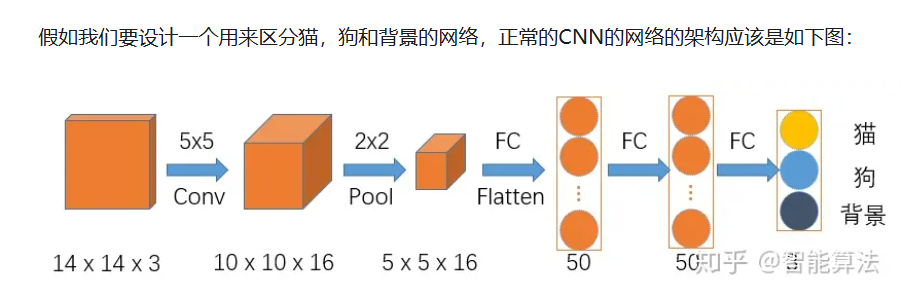
\includegraphics{CCN.png}
\end{figure}
\begin{figure}
    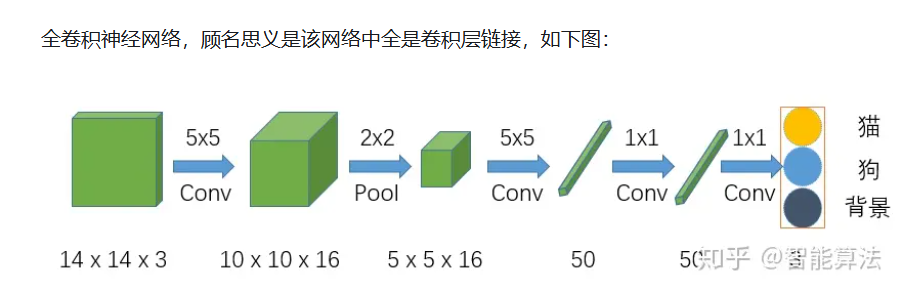
\includegraphics{FCN.png}
\end{figure}
而我们可以将全连接层中的操作理解为通过1*1的卷积层,并且最后的输出操作是一个矩阵,每一个点反应的是它再=在卷积操作中的涉及区域,相当于对输入图像进行了一个区域的分类,
且不再要求输入图像的尺寸大小固定
\end{document}